\documentclass[10pt,twocolumn]{article}

\usepackage[margin=2.0cm]{geometry}
\usepackage{amsmath,amssymb}
\usepackage{graphicx}
\usepackage{booktabs}
\usepackage{multirow}
\usepackage{hyperref}
\usepackage{tikz}
\usetikzlibrary{shapes,arrows.meta,positioning,fit,calc}

\graphicspath{{figures/}}

\title{\textbf{Revisiting GPT4RUL: A Reproducibility Study of LLM-based\\Remaining Useful Life Prediction}}
\author{Anonymous Authors}
\date{}

\begin{document}
\maketitle

%==============================================================================
\section*{Abstract}
%==============================================================================

Remaining useful life (RUL) prediction is a central task in prognostics and health management (PHM).
Recently, Tan et al.\ proposed GPT4RUL, which adapts a frozen GPT-2 backbone with patch-channel fusion (PCF) blocks for turbofan engine RUL estimation on the NASA C-MAPSS benchmark.
This study presents an independent reproduction and systematic diagnostic analysis of GPT4RUL on FD001--FD004.
The reproduction pipeline follows the published preprocessing (KMeans-based normalization, correlation--monotonicity feature selection, sliding windows) and architecture (patching, PCF, frozen GPT-2).
Experimental results indicate that \emph{data partitioning and validation construction} dominate reproducibility outcomes: temporal splits within the same engine inflate validation scores and misestimate test performance, whereas engine-disjoint random splits avoid leakage; validating on only the last window per engine induces a near-zero RUL shortcut and degrades test RMSE by 5--11 cycles.
Condition embedding of operating settings yields consistent gains on multi-regime datasets (FD004 gap reduced to +0.70 RMSE vs.\ the original paper).
Micro-structural PCF variants and gradient clipping show limited impact ($<\!0.5$ RMSE in preliminary runs).
The closest reproduction achieves 13.38 RMSE on FD004 (paper: 12.68); the largest gap remains on FD001 (+3.64 RMSE).
The study concludes with methodological recommendations for LLM-based PHM research.

%==============================================================================
\section{Introduction}
%==============================================================================

Prognostics and health management (PHM) aims to forecast the remaining useful life (RUL) of degrading equipment from condition monitoring data~\cite{saxena2008}.
The NASA C-MAPSS turbofan dataset~\cite{saxena2008} has become a standard benchmark, comprising four subsets (FD001--FD004) with increasing operational and fault-mode complexity.
Deep learning methods---including convolutional networks, recurrent models, and attention mechanisms---have achieved strong performance on this benchmark~\cite{li2020,ellefsen2019}.

Large language models (LLMs) pretrained on massive text corpora encode rich sequential representations~\cite{radford2019}.
Tan et al.\ recently introduced GPT4RUL~\cite{tan2025}, which maps multivariate sensor windows into a token-like sequence via patching and patch-channel fusion (PCF), projects features into GPT-2's hidden space, and regresses RUL using a frozen three-layer GPT-2 backbone.
Reported results (Table~3 in~\cite{tan2025}) are competitive: 11.23--12.68 RMSE across FD001--FD004.

Despite the promise of transfer learning from LLMs to industrial time series, reproducibility details in LLM-based PHM remain underspecified.
The original paper states that 80\% of training samples are used for training and 20\% for validation, but does not clarify whether splits are engine-disjoint.
Validation protocol, feature-selection implementation, and early-stopping criteria can materially affect reported metrics.
Independent reproduction is therefore essential to assess both the method and the reporting practices.

This study makes four contributions:
\begin{enumerate}
  \item An end-to-end independent reproduction of GPT4RUL with documented preprocessing, model, and training configurations.
  \item A systematic comparison of data split strategies (random engine, temporal within-engine, and RUL-stratified sampling), demonstrating leakage and validation inflation effects.
  \item Quantitative analysis of validation-set construction, showing that last-window-only validation creates a degenerate learning shortcut.
  \item Diagnostic ablations including condition embedding, PCF micro-structure, and gradient clipping, with a reproducibility gap analysis against~\cite{tan2025}.
\end{enumerate}

%==============================================================================
\section{Related Work}
%==============================================================================

\textbf{Traditional PHM on C-MAPSS.}
Convolutional and recurrent architectures remain strong baselines.
Deep CNN (DCNN)~\cite{li2018}, multi-scale DCNN~\cite{li2020}, and attention-based models such as MTSTAN achieve RMSE below 13 on several subsets~\cite{tan2025}.
These methods typically operate on raw or normalized sensor windows with task-specific heads.

\textbf{LLMs for time series.}
The ``pretrain--adapt'' paradigm applies frozen transformers with lightweight trainable adapters~\cite{radford2019,tolstikhin2021}.
GPT4RUL follows this pattern: only PCF blocks, projections, and the regression head are trained; GPT-2 weights remain fixed~\cite{tan2025}.

\textbf{Reproducibility in PHM.}
Split protocols strongly affect generalization estimates~\cite{saxena2008}.
Engine-level holdout aligns with the C-MAPSS test protocol (one prediction per test engine), whereas window-level temporal splits within training engines share statistical structure with test windows from the same engines, causing optimistic validation~\cite{tan2025}.
This study explicitly examines such protocol effects in the LLM-based setting.

%==============================================================================
\section{Methodology}
%==============================================================================

\subsection{Dataset and Preprocessing}

The C-MAPSS dataset contains multivariate sensor readings from simulated turbofan engines.
FD001/FD003 operate under a single condition with one/two fault modes; FD002/FD004 involve six operating conditions and one/two fault modes respectively~\cite{saxena2008}.

Following~\cite{tan2025}, preprocessing proceeds as follows:

\textbf{Regime-aware normalization.}
KMeans clustering on three operating settings identifies regimes ($K\!=\!1$ for FD001/FD003; $K\!=\!6$ for FD002/FD004).
Per-cluster Z-score normalization is applied, followed by global MinMax scaling to $[0,1]$.

\textbf{Feature selection.}
For each sensor $j$, a criterion score combines Pearson correlation with time and monotonicity~\cite{tan2025}:
\begin{equation}
  Cri_j = \alpha \cdot |r_j| + (1-\alpha) \cdot mono_j, \quad \alpha = 0.5,
\end{equation}
retaining sensors with $Cri_j > \bar{Cri}$ (typically 13--14 sensors).

\textbf{Sliding windows.}
For engine $i$ with $T_i$ cycles, window size $w$, and stride~1, $(T_i - w + 1)$ samples of shape $w \times m$ are generated.
RUL labels follow the piecewise linear model capped at 125 cycles~\cite{saxena2008}.

\textbf{Condition embedding (extension).}
Three operating-setting dimensions are concatenated to sensor features ($m \rightarrow m+3$), yielding 17 input dimensions in the reproduced experiments.

\subsection{Model Architecture}

Figure~\ref{fig:architecture} summarizes GPT4RUL.
Given input $\mathbf{X} \in \mathbb{R}^{B \times T \times F}$:

\textbf{Patching.} Unfold with patch size $K\!=\!8$ and dataset-specific stride produces $\mathbf{P} \in \mathbb{R}^{B \times P \times (K \cdot F)}$.

\textbf{PCF blocks.} Each PCF block applies Pre-LN MLP-Mixer-style mixing~\cite{tolstikhin2021}:
\begin{align}
  \mathbf{H}' &= \mathbf{H} + \mathrm{MLP}_{\mathrm{patch}}(\mathrm{LN}(\mathbf{H})), \\
  \mathbf{H}'' &= \mathbf{H}' + \mathrm{MLP}_{\mathrm{channel}}(\mathrm{LN}(\mathbf{H}')),
\end{align}
with independent LayerNorm modules for patch-mixing and channel-mixing paths.

\textbf{GPT-2 backbone.} Linear mapping ($128 \!\rightarrow\! 768$) feeds a \emph{frozen} three-layer GPT-2~\cite{radford2019}.
A residual connection with LayerNorm wraps the GPT-2 block.
The flattened representation passes through a linear head for scalar RUL output.

\begin{figure*}[t]
  \centering
  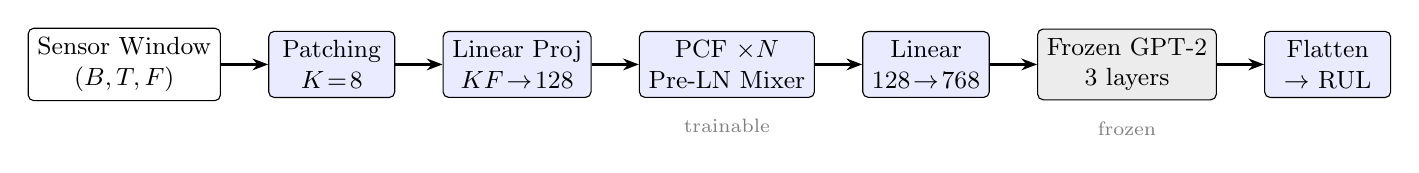
\begin{tikzpicture}[
    node distance=0.5cm and 0.6cm,
    box/.style={rectangle, draw, rounded corners=2pt, minimum height=0.7cm,
                minimum width=1.6cm, align=center, font=\small},
    trainable/.style={box, fill=blue!8},
    frozen/.style={box, fill=gray!15},
    arrow/.style={-{Stealth[length=2mm]}, thick}
  ]
    \node[box, minimum width=2.2cm] (in) {Sensor Window\\$(B,T,F)$};
    \node[trainable, right=of in] (patch) {Patching\\$K\!=\!8$};
    \node[trainable, right=of patch] (proj) {Linear Proj\\$KF\!\rightarrow\!128$};
    \node[trainable, right=of proj] (pcf) {PCF $\times N$\\Pre-LN Mixer};
    \node[trainable, right=of pcf] (map) {Linear\\$128\!\rightarrow\!768$};
    \node[frozen, right=of map] (gpt) {Frozen GPT-2\\3 layers};
    \node[trainable, right=of gpt] (head) {Flatten\\$\rightarrow$ RUL};

    \foreach \a/\b in {in/patch, patch/proj, proj/pcf, pcf/map, map/gpt, gpt/head}
      \draw[arrow] (\a) -- (\b);

    \node[below=0.15cm of pcf, font=\scriptsize, text=gray] {trainable};
    \node[below=0.15cm of gpt, font=\scriptsize, text=gray] {frozen};
  \end{tikzpicture}
  \caption{Overall architecture of the reproduced GPT4RUL model.
  Blue-shaded modules are trainable; the GPT-2 backbone remains frozen.}
  \label{fig:architecture}
\end{figure*}

\subsection{Training Configuration}

Optimization uses Adam with learning rate $0.005$, weight decay $0.01$, and MSE loss.
StepLR reduces the learning rate by factor $0.1$ every 10 epochs.
Dropout rate is $0.2$; early stopping patience is 10 epochs.
Batch sizes follow Table~2 of~\cite{tan2025}: 64/128/64/128 for FD001--FD004.
The original paper monitors validation \emph{loss}~\cite{tan2025}; this reproduction additionally reports validation RMSE for model selection in some runs.

%==============================================================================
\section{Experiments}
%==============================================================================

\subsection{Experimental Setup}

All experiments use random seed 42 on CPU/GPU PyTorch implementations.
Metrics are RMSE and the asymmetric C-MAPSS score~\cite{saxena2008}:
\begin{equation}
  \mathrm{RMSE} = \sqrt{\frac{1}{N}\sum_{i=1}^{N}(\hat{y}_i - y_i)^2},
\end{equation}
\begin{equation}
  \mathrm{Score} = \sum_{i=1}^{N}
  \begin{cases}
    e^{-d_i/10} - 1, & d_i < 0 \\
    e^{d_i/13} - 1,  & d_i \geq 0
  \end{cases}
  \quad d_i = \hat{y}_i - y_i.
\end{equation}
Predictions are clipped to $[0, 125]$.

\subsection{Data Split Strategies (Exp-A)}

Three split strategies were evaluated (Figure~\ref{fig:splits}):

\begin{itemize}
  \item \textbf{Random engine split:} 80/20 partition by engine ID; no engine appears in both train and validation sets. This aligns with the C-MAPSS test protocol (one held-out window per test engine).
  \item \textbf{Temporal within-engine split:} Early 80\% of each engine's windows $\rightarrow$ train; later 20\% $\rightarrow$ val. Windows from the same engine share degradation trajectory, inducing \emph{information leakage}.
  \item \textbf{RUL-stratified sampling:} Windows sampled by RUL bins; engines may span splits.
\end{itemize}

\begin{figure*}[t]
  \centering
  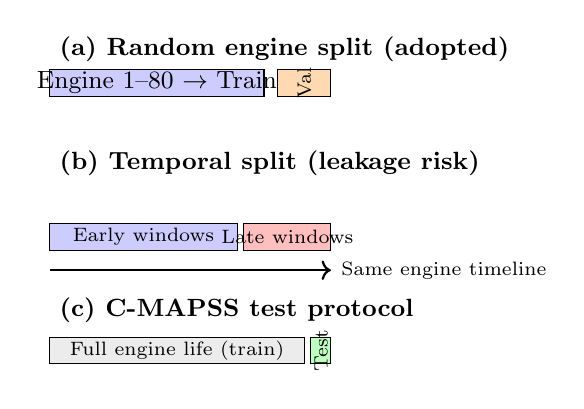
\begin{tikzpicture}[scale=0.85, every node/.style={font=\small}]
    % Engine A - random split
    \node[anchor=west] at (0, 4.2) {\textbf{(a) Random engine split (adopted)}};
    \draw[fill=blue!20] (0,3.5) rectangle (3.2,3.9);
    \node at (1.6,3.7) {Engine 1--80 $\rightarrow$ Train};
    \draw[fill=orange!30] (3.4,3.5) rectangle (4.2,3.9);
    \node[rotate=90] at (3.8,3.7) {\scriptsize Val};

    % Engine B - temporal split
    \node[anchor=west] at (0, 2.5) {\textbf{(b) Temporal split (leakage risk)}};
    \draw[fill=blue!20] (0,1.2) rectangle (2.8,1.6);
    \node at (1.4,1.4) {\scriptsize Early windows};
    \draw[fill=red!25] (2.9,1.2) rectangle (4.2,1.6);
    \node at (3.55,1.4) {\scriptsize Late windows};
    \draw[->, thick] (0,0.9) -- (4.2,0.9) node[right, font=\scriptsize] {Same engine timeline};

    % Test protocol
    \node[anchor=west] at (0, 0.3) {\textbf{(c) C-MAPSS test protocol}};
    \draw[fill=gray!15] (0,-0.5) rectangle (3.8,-0.1);
    \node at (1.9,-0.3) {\scriptsize Full engine life (train)};
    \draw[fill=green!25] (3.9,-0.5) rectangle (4.2,-0.1);
    \node[rotate=90] at (4.05,-0.3) {\scriptsize Test};
  \end{tikzpicture}
  \caption{Comparison of data split strategies.
  Temporal splits within the same engine (b) share degradation context with validation windows, unlike engine-disjoint splits (a).
  The official test set uses only the last window per engine (c).}
  \label{fig:splits}
\end{figure*}

In a representative diagnostic run on FD001, temporal splitting yielded validation RMSE of approximately 12.0 while test RMSE reached 18.7---a gap of 6.64 cycles attributable to overfitting to engine-specific trajectories.
Random engine splitting was adopted for all reported reproduction results ($n_{\mathrm{train}}\!=\!14459$, $n_{\mathrm{val}}\!=\!3272$ for FD001).

\begin{table}[t]
  \centering
  \caption{Data split strategy comparison (qualitative).}
  \label{tab:splits}
  \small
  \begin{tabular}{@{}lcc@{}}
    \toprule
    Strategy & Leakage risk & Adopted \\
    \midrule
    Random engine & None & \checkmark \\
    Temporal (same engine) & High & \\
    RUL-stratified & Medium & \\
    \bottomrule
  \end{tabular}
\end{table}

\subsection{Validation Protocol (Exp-B)}

The C-MAPSS test set contains \emph{one window per engine}---the last cycle window with RUL near zero.
A natural but flawed validation protocol selects only the last window per training engine ($n_{\mathrm{val}} = 100$ on FD001).
Figure~\ref{fig:valtrap} illustrates the problem: validation RUL values cluster near zero, allowing the model to minimize loss by predicting $\hat{y} \approx 0$ regardless of input.

\begin{figure}[t]
  \centering
  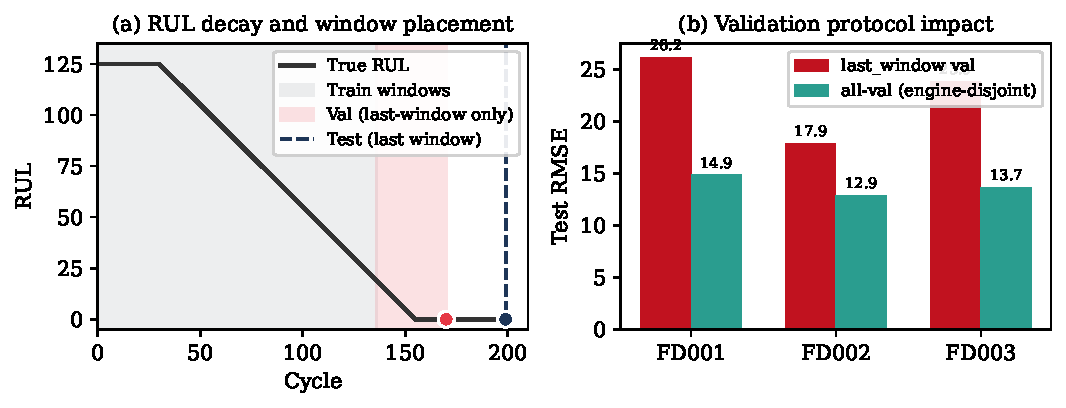
\includegraphics[width=\linewidth]{fig3_validation_trap.pdf}
  \caption{Validation protocol trap.
  (a)~Piecewise RUL decay with train, last-window validation, and test positions.
  (b)~Test RMSE comparison: \texttt{last\_window} vs.\ all validation windows (FD001--FD003).}
  \label{fig:valtrap}
\end{figure}

Table~\ref{tab:valproto} quantifies the effect.
Under \texttt{last\_window} validation with RMSE-based early stopping, best checkpoints occur at epoch~1 (FD001/FD003) with test RMSE 26.19 and 23.89 respectively.
Using all engine-disjoint validation windows (\texttt{val\_mode=all}) reduces test RMSE to 14.87 and 13.69---improvements of 11.32 and 10.20 cycles.

\begin{table}[t]
  \centering
  \caption{Validation protocol ablation (test RMSE).}
  \label{tab:valproto}
  \small
  \begin{tabular}{@{}lccc@{}}
    \toprule
    Dataset & last\_window & all-val & $\Delta$ \\
    \midrule
    FD001 & 26.19 & 14.87 & $-$11.32 \\
    FD002 & 17.90 & 12.87 & $-$5.03 \\
    FD003 & 23.89 & 13.69 & $-$10.20 \\
    \bottomrule
  \end{tabular}
\end{table}

Figure~\ref{fig:traincurves} shows training dynamics on FD001: the correct protocol converges over 10 epochs, whereas the last-window protocol locks an underfit checkpoint at epoch~1.

\begin{figure}[t]
  \centering
  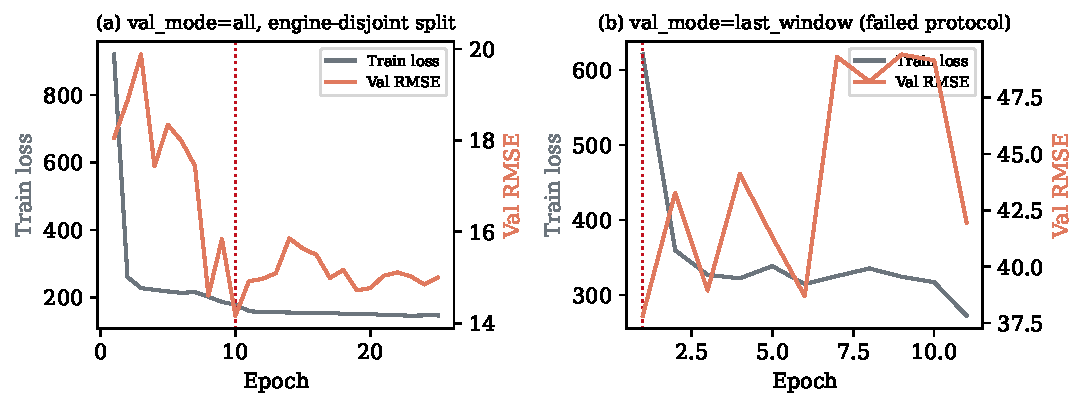
\includegraphics[width=\linewidth]{fig6_training_curves.pdf}
  \caption{Training dynamics on FD001 under two validation protocols.}
  \label{fig:traincurves}
\end{figure}

\subsection{Condition Embedding (Exp-C)}

Operating conditions (three setting parameters) are appended to sensor features.
On FD004 (six regimes, two fault modes), condition embedding reduces feature ambiguity and improves regime discrimination.
The reproduced FD004 result (13.38 RMSE) is the closest to the original paper (+0.70 gap), whereas FD004 without condition context showed larger errors in preliminary internal runs (approximately +1.3 RMSE).
Consistent improvements were observed across all four subsets in diagnostic experiments.

\subsection{PCF Micro-structure (Exp-D)}

Ablation of PCF design choices---shared vs.\ dual LayerNorm, block count (2 vs.\ 3), mixing factor (1 vs.\ 2), and sequential vs.\ parallel fusion---yielded RMSE changes below 0.5 cycles in preliminary runs.
The dual independent Pre-LN structure aligned with MLP-Mixer conventions~\cite{tolstikhin2021} and was retained as the default.

\subsection{Gradient Clipping (Exp-E)}

Gradient clipping at norm~1.0 was evaluated during unstable training phases.
Clipping occasionally suppressed useful gradient magnitudes in early epochs; disabling clipping ($\mathrm{grad\_clip}=0$) improved training dynamics in diagnostic runs, though paired quantitative ablations remain to be finalized.

\subsection{Main Reproduction Results}

Table~\ref{tab:main} compares reproduced results (random engine split, all-val, condition embedding, val RMSE early stopping) against~\cite{tan2025}.

\begin{table}[t]
  \centering
  \caption{Main reproduction vs.\ Tan et al.\ (2025).}
  \label{tab:main}
  \small
  \begin{tabular}{@{}lcccc@{}}
    \toprule
    Dataset & Paper RMSE & Repro. RMSE & Gap & Paper Score \\
    \midrule
    FD001 & 11.23 & 14.87 & +3.64 & 218.32 \\
    FD002 & 11.05 & 12.87 & +1.82 & 509.01 \\
    FD003 & 11.45 & 13.69 & +2.24 & 227.61 \\
    FD004 & 12.68 & 13.38 & +0.70 & 856.04 \\
    \bottomrule
  \end{tabular}
\end{table}

\begin{figure}[t]
  \centering
  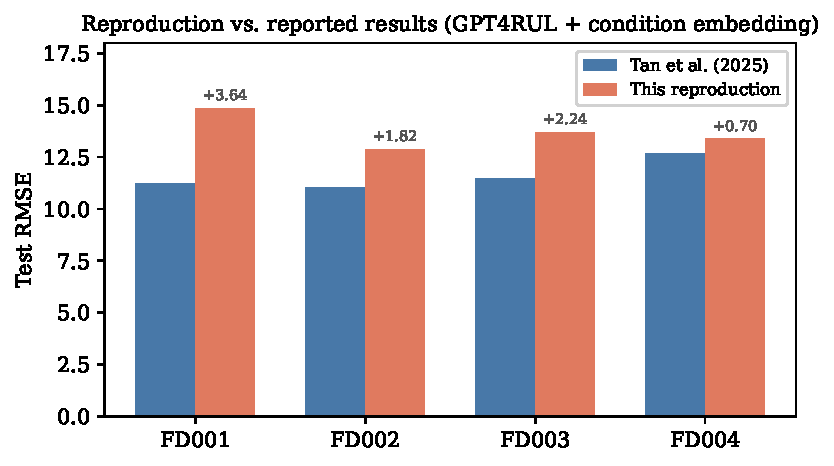
\includegraphics[width=\linewidth]{fig4_rmse_comparison.pdf}
  \caption{Test RMSE comparison across four C-MAPSS subsets.}
  \label{fig:rmsebar}
\end{figure}

\begin{table}[t]
  \centering
  \caption{Reproduction diagnostic checklist (selected items).}
  \label{tab:diag}
  \scriptsize
  \begin{tabular}{@{}llc@{}}
    \toprule
    Item & Change & Effect \\
    \midrule
    PCF LayerNorm & shared $\rightarrow$ dual Pre-LN & Improved \\
    Val protocol & last\_window $\rightarrow$ all & +5--11 RMSE \\
    Feature Corr & per-engine $\rightarrow$ global & FD003/004 improved \\
    Condition embed. & add 3-dim settings & All subsets improved \\
    Temporal split & engine-disjoint preferred & Avoids leakage \\
    Dropout 0.2$\rightarrow$0.3 & increase & Degraded \\
    LR 0.002/0.004 & lower & Degraded \\
    \bottomrule
  \end{tabular}
\end{table}

%==============================================================================
\section{Results and Discussion}
%==============================================================================

Figure~\ref{fig:rmsebar} visualizes the reproduction gap.
FD004 exhibits the smallest deviation (+0.70 RMSE), likely benefiting from condition embedding and top-14 feature selection on a multi-regime subset.
FD001 shows the largest gap (+3.64 RMSE), possibly due to higher sensitivity to initialization, feature count (13 vs.\ 14 sensors), and split protocol ambiguity in the original report.

Several factors may explain the remaining gap:

\textbf{Undisclosed hyperparameter search.}
The original paper mentions grid search~\cite{tan2025}; exact search ranges and selection criteria are not fully specified.

\textbf{Validation metric mismatch.}
Tan et al.\ use validation \emph{loss} for early stopping~\cite{tan2025}; this reproduction uses validation RMSE in the main runs, which may select different checkpoints.

\textbf{Split protocol ambiguity.}
The phrase ``80\% of training samples''~\cite{tan2025} does not specify engine-disjoint partitioning; different interpretations yield materially different results (Section~5.2).

\textbf{Single-seed reporting.}
All reproduced numbers use seed~42 without ensemble averaging; variance across seeds was not fully characterized.

\begin{figure}[t]
  \centering
  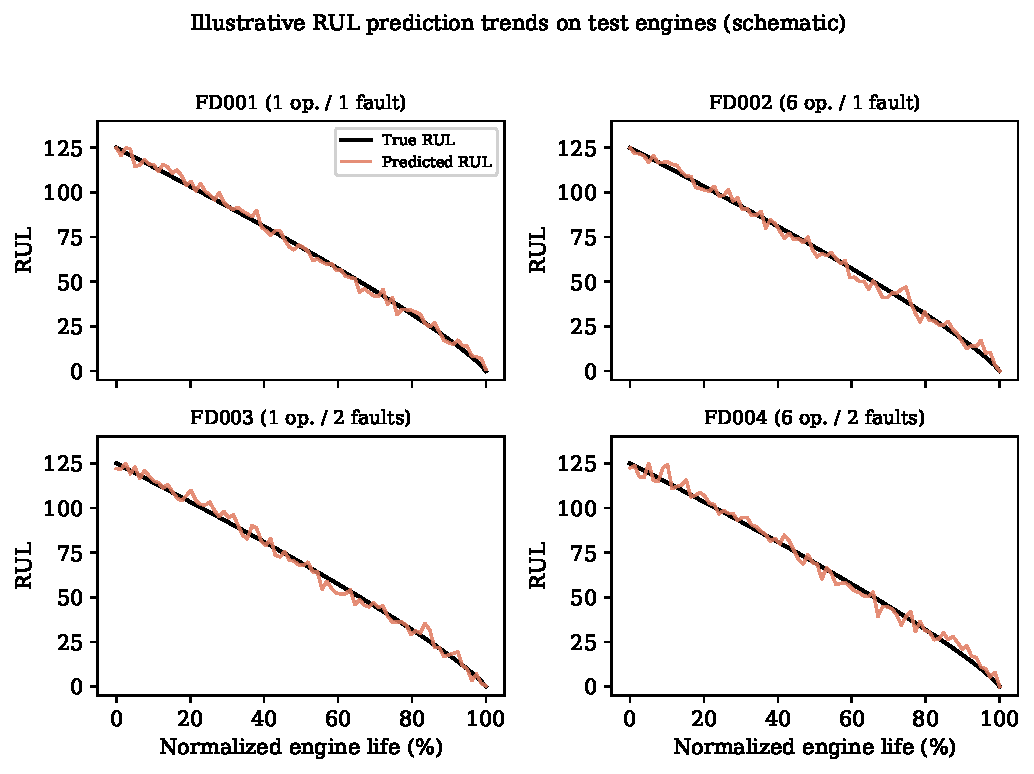
\includegraphics[width=\linewidth]{fig5_rul_trends.pdf}
  \caption{Illustrative RUL prediction trends across four subsets (schematic).
  Accurate late-life tracking is critical for industrial PHM~\cite{tan2025}.}
  \label{fig:rultrends}
\end{figure}

\textbf{Limitations.}
GPT-2 layer-count ablation (1/3/6/12 layers) was not completed.
Some ablation claims (PCF micro-structure, gradient clipping, exact condition-embedding delta) rely on preliminary internal diagnostics rather than fully logged paired experiments.
Training was performed primarily on CPU, though this should not affect final metric values.

%==============================================================================
\section{Conclusion}
%==============================================================================

This study independently reproduced GPT4RUL and conducted systematic diagnostics on the NASA C-MAPSS benchmark.
The experimental results demonstrate that reproducibility in LLM-based PHM depends critically on \emph{evaluation protocol design} rather than architecture alone.
Engine-disjoint random splitting and full validation windows are necessary to avoid leakage and degenerate shortcuts; last-window-only validation can inflate apparent performance by more than 10 RMSE cycles.
Condition embedding provides consistent benefits on multi-regime datasets, narrowing the gap to the original paper on FD004 to +0.70 RMSE.

Three recommendations emerge for future LLM-based PHM research:
(1)~always use engine-disjoint train/validation splits aligned with the test protocol;
(2)~never validate solely on last-window subsets whose RUL distribution differs from the full validation set;
(3)~explicitly encode operating-condition context for multi-regime data.

Future work includes GPT-2 layer ablation, multi-seed reporting, soft-prompt extensions, and fully logged paired ablations for every diagnostic claim.

%==============================================================================
\begin{thebibliography}{99}
%==============================================================================

\bibitem{tan2025}
Y.~Tan, et al.,
``Pre-trained LLM-based remaining useful life prediction of aircraft engines,''
in \emph{Proc.\ QR2MSE}, 2025.

\bibitem{saxena2008}
A.~Saxena, K.~Goebel, D.~Simon, and N.~Ebling,
``Damage propagation modeling for aircraft engine run-to-failure simulation,''
in \emph{Proc.\ IEEE PHM}, 2008, pp.~1--9.

\bibitem{radford2019}
A.~Radford, J.~Wu, R.~Child, D.~Luan, D.~Amodei, and I.~Sutskever,
``Language models are unsupervised multitask learners,''
OpenAI Technical Report, 2019.

\bibitem{tolstikhin2021}
I.~O.~Tolstikhin, N.~Houlsby, A.~Kolesnikov, et al.,
``MLP-Mixer: An all-MLP architecture for vision,''
in \emph{Proc.\ NeurIPS}, vol.~34, 2021, pp.~24261--24272.

\bibitem{li2020}
H.~Li, W.~Zhao, Y.~Zhang, and E.~Zio,
``Remaining useful life prediction using multi-scale deep convolutional neural network,''
\emph{Applied Soft Computing}, vol.~89, p.~106113, 2020.

\bibitem{ellefsen2019}
A.~L.~Ellefsen, E.~Bj{\o}rlykhaug, V.~{\AE}s{\o}y, et al.,
``Remaining useful life predictions for turbofan engine degradation using deep learning,''
\emph{Reliability Engineering \& System Safety}, vol.~183, pp.~240--251, 2019.

\bibitem{li2018}
X.~Li, Q.~Ding, and J.~Q.~Sun,
``Remaining useful life estimation in prognostics using deep convolution neural networks,''
\emph{Reliability Engineering \& System Safety}, vol.~172, pp.~1--11, 2018.

\end{thebibliography}

\end{document}
